\documentclass[a4paper]{article}
\usepackage{ctex}
\usepackage{listings}
\usepackage{xcolor}
\usepackage{fancyhdr}
\usepackage{graphicx}
\graphicspath{ {pic/} }
\pagestyle{fancy}
\rhead{Mingchen Liu}
\lstset{
    %backgroundcolor=\color{red!50!green!50!blue!50},%代码块背景色为浅灰色
    rulesepcolor= \color{gray}, %代码块边框颜色
    breaklines=true,  %代码过长则换行
    numbers=left, %行号在左侧显示
    numberstyle= \small,%行号字体
    %keywordstyle= \color{red},%关键字颜色
    commentstyle=\color{gray}, %注释颜色
    frame=shadowbox%用方框框住代码块
    }

% Title
\title{TDD测试驱动开发实验}
\author{刘铭宸\\软件工程2003班\\U202010783}
\date{\today}
 
\begin{document}

\begin{titlepage}
\maketitle
\end{titlepage}

\tableofcontents

\newpage
\section{关于测试驱动开发}
\subsection{何谓测试驱动开发?}
正如《测试驱动开发》一书中所言,\emph{测试驱动开发(TDD)以测试作为开发过程的中心,它要求在编写任何产品代码之前,
首先编写用于定义产品代码行为的测试,而编写的产品代码又要以使测试通过为目标。测试驱动开发要求测试可以完全自动化地运行,在对代码进行重构前后必须运行测试。
这是一种革命性的开发方法,能够造就简单、清晰、高质量的代码。}
\subsection{为何要使用TDD?}
测试驱动开发的主要好处有以下这些:
\begin{enumerate}
    \item \emph{代码覆盖}。原则上讲,所编写的每个代码段都应当有至少一个相关的测试。这样,就可以有把握地相信系统中的所有代码都被执行过了。代码在编写时就会被测试,因此可以在开发过程中的早期发现缺陷。
    \item \emph{回归测试}。测试集随着程序的开发增量进行开发。可以总是运行回归测试来确认对程序的修改没有引入新的bug。
    \item \emph{简化的调试}。当一个测试失败时,问题出在哪里应该很明显。新写的代码需要进行检查和修改。不需要使用调试工具来定位问题。关于测试驱动开发的使用报告建议说,在测试驱动的开发中一般不需要使用自动化的调试器(Martin 2007)。
    \item \emph{系统文档化}。测试自身可以作为某种形式的文档来描述代码应该做什么。阅读测试可以使理解代码变得更容易。 
\end{enumerate}

\subsection{如何进行测试驱动开发?}
\begin{figure}[b]
    \centering
    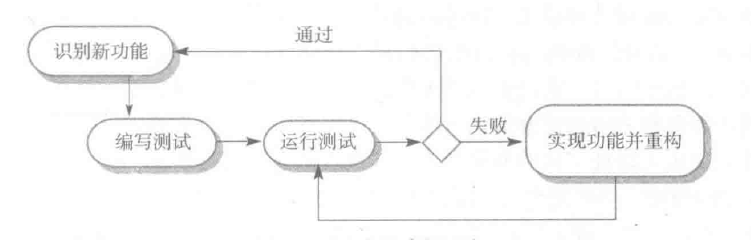
\includegraphics[scale=0.4]{pic01.png}
    \caption{测试驱动开发过程}
    \label{fig:1}
\end{figure}
\newpage

\section{实验内容——判断字符串是否是IPV4地址}
采用测试驱动开发方法,将需求分为5个子功能实现,并使用JUnit框架分别进行测试。
\subsection{判断字符串是否为空串}
\subsubsection*{编写测试}
\begin{figure}[h]
    \centering
    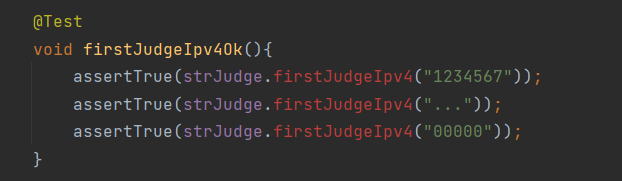
\includegraphics[scale=0.8]{1.1.png}
    \caption{正确用例测试}
    \label{fig:2}
\end{figure}
\begin{figure}[h]
    \centering
    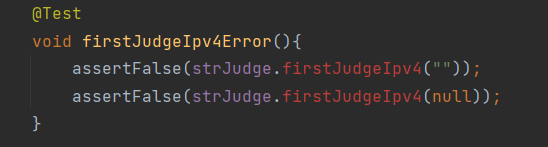
\includegraphics[scale=0.9]{1.2.png}
    \caption{错误用例测试}
    \label{fig:3}
\end{figure}
\subsubsection*{运行测试}
\begin{figure}[h]
    \centering
    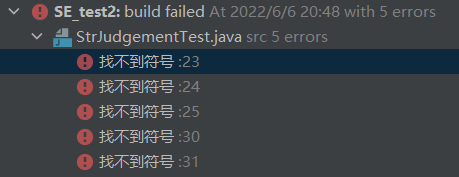
\includegraphics[scale=0.9]{1.3.png}
    \caption{第一次测试}
    \label{fig:4}
\end{figure}
由于该功能尚未实现,无法通过测试。
\subsubsection*{实现功能并重构}
\begin{figure}[h]
    \centering
    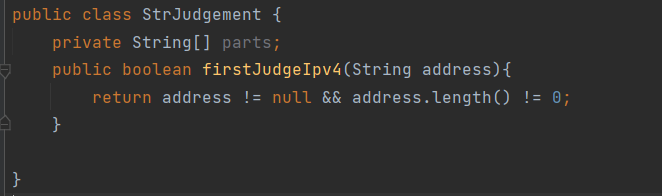
\includegraphics[scale=0.8]{1.4.png}
    \caption{实现功能并重构}
    \label{fig:5}
\end{figure}
\subsubsection*{再次运行测试}
\begin{figure}[h]
    \centering
    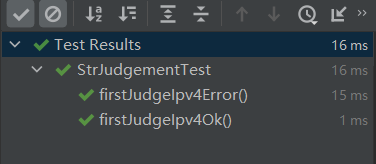
\includegraphics[scale=0.9]{1.5.png}
    \caption{第二次测试}
    \label{fig:6}
\end{figure}
测试通过

\subsection{判断字符串是否可被.分成四段}
\subsubsection*{编写测试}
\begin{figure}[h]
    \centering
    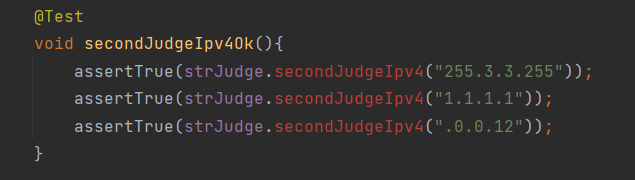
\includegraphics[scale=0.8]{2.1.png}
    \caption{正确用例测试}
    \label{fig:7}
\end{figure}
\begin{figure}[h]
    \centering
    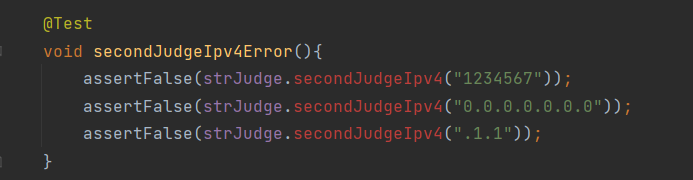
\includegraphics[scale=0.8]{2.2.png}
    \caption{错误用例测试}
    \label{fig:8}
\end{figure}
~\\
\subsubsection*{运行测试}
\begin{figure}[h]
    \centering
    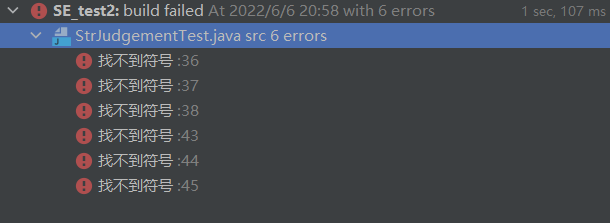
\includegraphics[scale=0.9]{2.3.png}
    \caption{第一次测试}
    \label{fig:9}
\end{figure}
由于该功能尚未实现,无法通过测试。
\subsubsection*{实现功能并重构}
\begin{figure}[h]
    \centering
    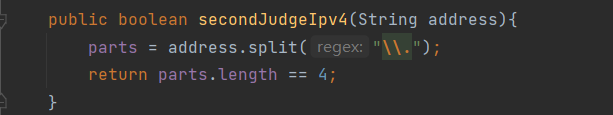
\includegraphics[scale=0.8]{2.4.png}
    \caption{实现功能并重构}
    \label{fig:10}
\end{figure}
~\\~\\~\\~\\~\\
\subsubsection*{再次运行测试}
\begin{figure}[h]
    \centering
    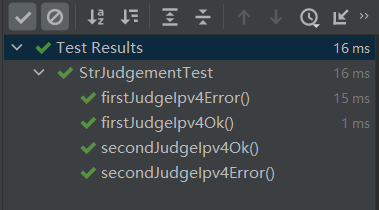
\includegraphics[scale=0.9]{2.5.png}
    \caption{第二次测试}
    \label{fig:11}
\end{figure}
测试通过

\subsection{判断每一段是否是在0到255之间的数字}
\subsubsection*{编写测试}
\begin{figure}[h]
    \centering
    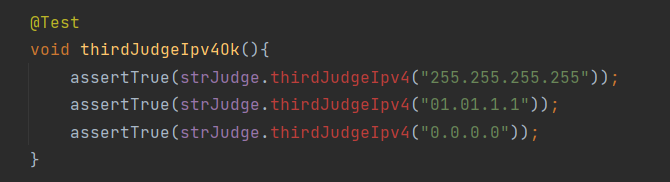
\includegraphics[scale=0.8]{3.1.png}
    \caption{正确用例测试}
    \label{fig:12}
\end{figure}
\begin{figure}[h]
    \centering
    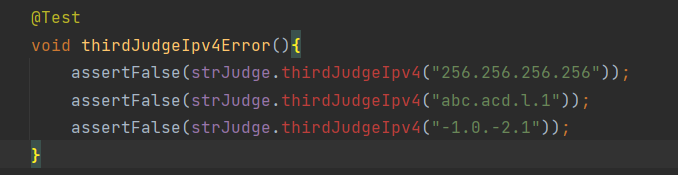
\includegraphics[scale=0.8]{3.2.png}
    \caption{错误用例测试}
    \label{fig:13}
\end{figure}
~\\~\\
\subsubsection*{运行测试}
\begin{figure}[h]
    \centering
    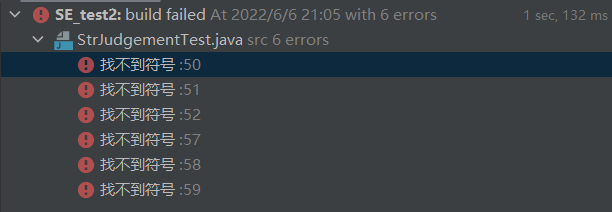
\includegraphics[scale=0.9]{3.3.png}
    \caption{第一次测试}
    \label{fig:14}
\end{figure}
由于该功能尚未实现,无法通过测试。
\subsubsection*{实现功能并重构}
\begin{figure}[h]
    \centering
    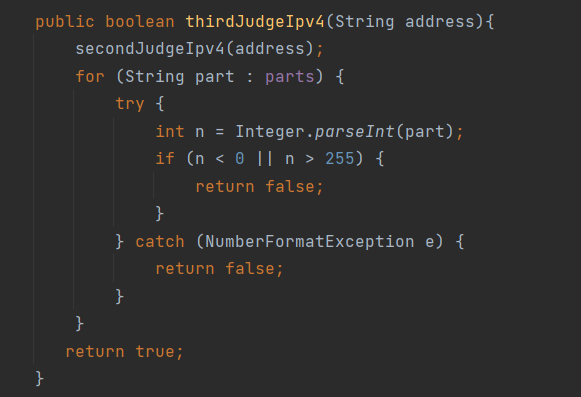
\includegraphics[scale=0.8]{3.4.png}
    \caption{实现功能并重构}
    \label{fig:15}
\end{figure}
~\\~\\~\\~\\~\\
\subsubsection*{再次运行测试}
\begin{figure}[h]
    \centering
    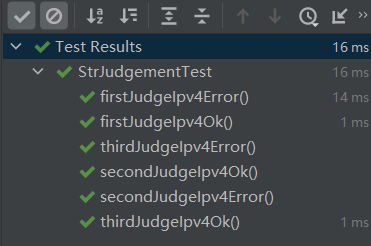
\includegraphics[scale=0.9]{3.5.png}
    \caption{第二次测试}
    \label{fig:16}
\end{figure}
测试通过

\subsection{判断是否存在以0开头的非零数字}
\subsubsection*{编写测试}
\begin{figure}[h]
    \centering
    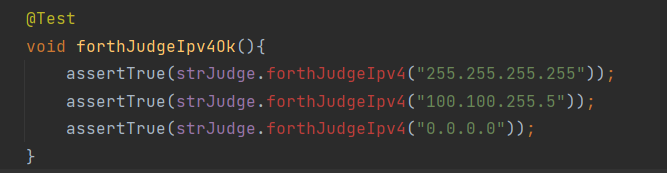
\includegraphics[scale=0.8]{4.1.png}
    \caption{正确用例测试}
    \label{fig:17}
\end{figure}
\begin{figure}[h]
    \centering
    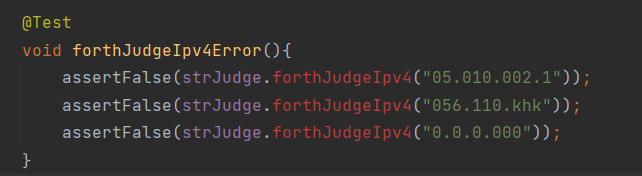
\includegraphics[scale=0.8]{4.2.png}
    \caption{错误用例测试}
    \label{fig:18}
\end{figure}
~\\
\subsubsection*{运行测试}
\begin{figure}[h]
    \centering
    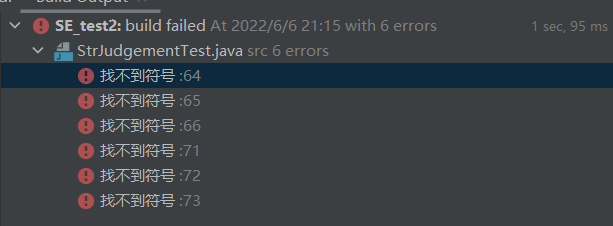
\includegraphics[scale=0.9]{4.3.png}
    \caption{第一次测试}
    \label{fig:19}
\end{figure}
由于该功能尚未实现,无法通过测试。
\subsubsection*{实现功能并重构}
\begin{figure}[h]
    \centering
    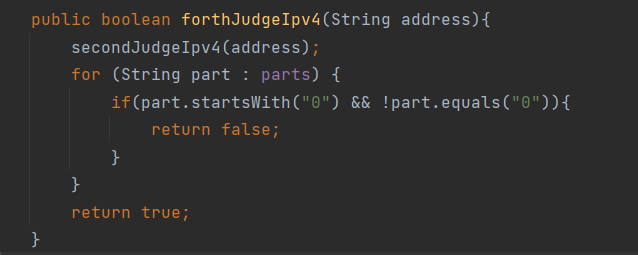
\includegraphics[scale=0.8]{4.4.png}
    \caption{实现功能并重构}
    \label{fig:20}
\end{figure}
~\\~\\~\\~\\~\\~\\~\\~\\
\subsubsection*{再次运行测试}
\begin{figure}[h]
    \centering
    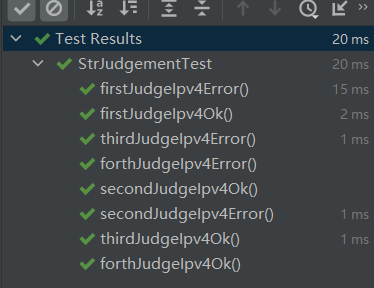
\includegraphics[scale=0.9]{4.5.png}
    \caption{第二次测试}
    \label{fig:21}
\end{figure}
测试通过

\subsection{判断字符串是否同时满足上述条件}
\subsubsection*{编写测试}
\begin{figure}[h]
    \centering
    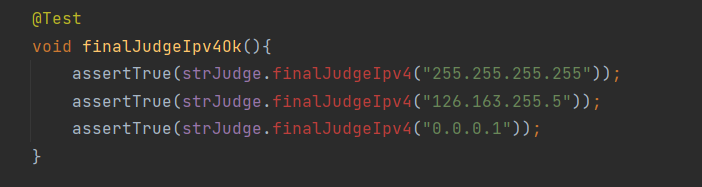
\includegraphics[scale=0.7]{5.1.png}
    \caption{正确用例测试}
    \label{fig:22}
\end{figure}
\begin{figure}[h]
    \centering
    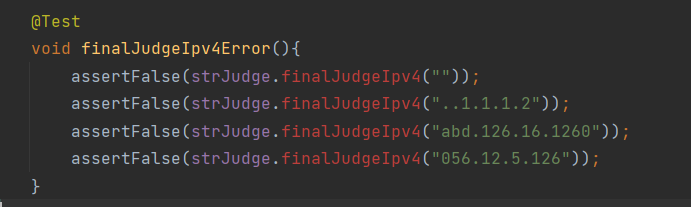
\includegraphics[scale=0.7]{5.2.png}
    \caption{错误用例测试}
    \label{fig:23}
\end{figure}
~\\
\subsubsection*{运行测试}
\begin{figure}[h]
    \centering
    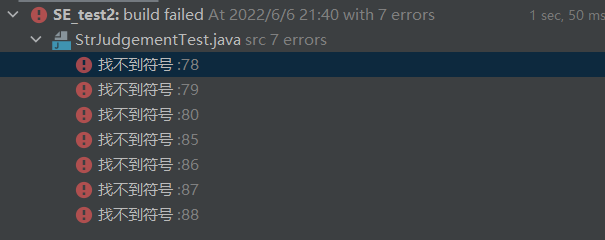
\includegraphics[scale=0.9]{5.3.png}
    \caption{第一次测试}
    \label{fig:24}
\end{figure}
由于该功能尚未实现,无法通过测试。
\subsubsection*{实现功能并重构}
\begin{figure}[h]
    \centering
    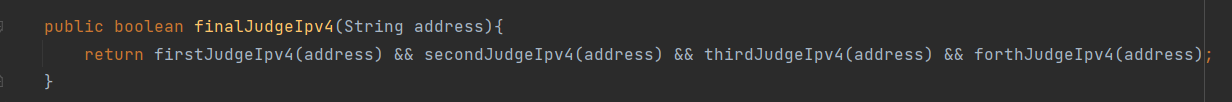
\includegraphics[scale=0.6]{5.6.png}
    \caption{实现功能并重构}
    \label{fig:25}
\end{figure}
\subsubsection*{再次运行测试}
\begin{figure}[h]
    \centering
    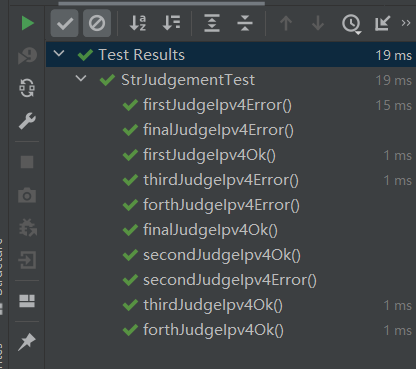
\includegraphics[scale=0.7]{5.7.png}
    \caption{第二次测试}
    \label{fig:26}
\end{figure}
测试通过

\section{代码展示}
\subsection{程序代码}
\begin{lstlisting}[language={java}]
    public class StrJudgement {
        private String[] parts;
        public boolean firstJudgeIpv4(String address){
            return address != null && address.length() != 0;
        }

        public boolean secondJudgeIpv4(String address){
            parts = address.split("\\.");
            return parts.length == 4;
        }

        public boolean thirdJudgeIpv4(String address){
            secondJudgeIpv4(address);
            for (String part : parts) {
                try {
                    int n = Integer.parseInt(part);
                    if (n < 0 || n > 255) {
                        return false;
                    }
                } catch (NumberFormatException e) {
                    return false;
                }
            }
            return true;
        }

        public boolean forthJudgeIpv4(String address){
            secondJudgeIpv4(address);
            for (String part : parts) {
                if(part.startsWith("0") && !part.equals("0")){
                    return false;
                }
            }
            return true;
        }

        public boolean finalJudgeIpv4(String address){
            return firstJudgeIpv4(address) && secondJudgeIpv4(address) && thirdJudgeIpv4(address) && forthJudgeIpv4(address);
        }
    }
\end{lstlisting}

\subsection{测试代码}
\begin{lstlisting}[language={java}]
    import org.junit.jupiter.api.AfterEach;
    import org.junit.jupiter.api.BeforeEach;
    import org.junit.jupiter.api.Test;
    import java.util.Arrays;
    import static org.junit.jupiter.api.Assertions.*;
    
    class StrJudgementTest {
        StrJudgement strJudge;
        @BeforeEach
        void setUp() {
            strJudge = new StrJudgement();
        }
    
        @AfterEach
        void tearDown() {
            strJudge = null;
        }
    
        @Test
        void firstJudgeIpv4Ok(){
            assertTrue(strJudge.firstJudgeIpv4("1234567"));
            assertTrue(strJudge.firstJudgeIpv4("..."));
            assertTrue(strJudge.firstJudgeIpv4("00000"));
        }
    
        @Test
        void firstJudgeIpv4Error(){
            assertFalse(strJudge.firstJudgeIpv4(""));
            assertFalse(strJudge.firstJudgeIpv4(null));
        }
    
        @Test
        void secondJudgeIpv4Ok(){
            assertTrue(strJudge.secondJudgeIpv4("255.3.3.255"));
            assertTrue(strJudge.secondJudgeIpv4("1.1.1.1"));
            assertTrue(strJudge.secondJudgeIpv4(".0.0.12"));
        }
    
        @Test
        void secondJudgeIpv4Error(){
            assertFalse(strJudge.secondJudgeIpv4("1234567"));
            assertFalse(strJudge.secondJudgeIpv4("0.0.0.0.0.0.0"));
            assertFalse(strJudge.secondJudgeIpv4(".1.1"));
        }
    
        @Test
        void thirdJudgeIpv4Ok(){
            assertTrue(strJudge.thirdJudgeIpv4("255.255.255.255"));
            assertTrue(strJudge.thirdJudgeIpv4("01.01.1.1"));
            assertTrue(strJudge.thirdJudgeIpv4("0.0.0.0"));
        }
    
        @Test
        void thirdJudgeIpv4Error(){
            assertFalse(strJudge.thirdJudgeIpv4("256.256.256.256"));
            assertFalse(strJudge.thirdJudgeIpv4("abc.acd.l.1"));
            assertFalse(strJudge.thirdJudgeIpv4("-1.0.-2.1"));
        }
    
        @Test
        void forthJudgeIpv4Ok(){
            assertTrue(strJudge.forthJudgeIpv4("255.255.255.255"));
            assertTrue(strJudge.forthJudgeIpv4("100.100.255.5"));
            assertTrue(strJudge.forthJudgeIpv4("0.0.0.0"));
        }
    
        @Test
        void forthJudgeIpv4Error(){
            assertFalse(strJudge.forthJudgeIpv4("05.010.002.1"));
            assertFalse(strJudge.forthJudgeIpv4("056.110.khk"));
            assertFalse(strJudge.forthJudgeIpv4("0.0.0.000"));
        }
    
        @Test
        void finalJudgeIpv4Ok(){
            assertTrue(strJudge.finalJudgeIpv4("255.255.255.255"));
            assertTrue(strJudge.finalJudgeIpv4("126.163.255.5"));
            assertTrue(strJudge.finalJudgeIpv4("0.0.0.1"));
        }
    
        @Test
        void finalJudgeIpv4Error(){
            assertFalse(strJudge.finalJudgeIpv4(""));
            assertFalse(strJudge.finalJudgeIpv4("..1.1.1.2"));
            assertFalse(strJudge.finalJudgeIpv4("abd.126.16.1260"));
            assertFalse(strJudge.finalJudgeIpv4("056.12.5.126"));
        }
    }
\end{lstlisting}
\section{参考资料}
[1]教学课件:感谢华中科技大学软件学院刘小峰老师!

[2](美)贝克(Kent Beck)著. 孙平平等译. 测试驱动开发. 北京:中国电力出版社. 2004

[3](英)伊恩$\cdot$萨默维尔(Ian Sommerville)著. 彭鑫等译. 软件工程(原书第10版). 北京:机械工业出版社. 2018
\end{document} 